\documentclass[12pt, letterpaper]{article}

\usepackage{amsmath}
\usepackage[a4paper, portrait, margin=1in]{geometry}
\usepackage{hyperref}
\usepackage{tikz}

\title{CSS601 Introduction to Artificial Intelligence - Assignment 2}
\author{Ian Chong Wei Ming\\\href{mailto:ian.chong.2020@mitb.smu.edu.sg}{ian.chong.2020@mitb.smu.edu.sg}}
\date{\today}

\begin{document}

\maketitle
\section{Heuristic Search}

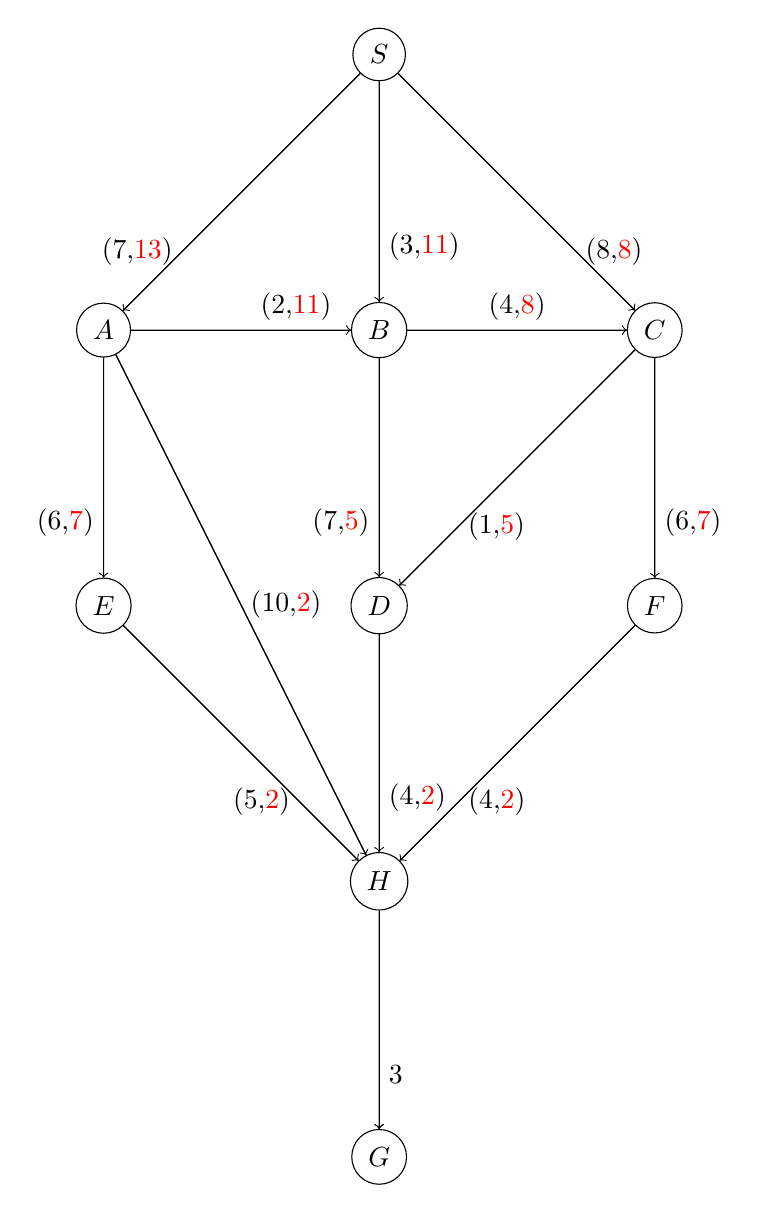
\begin{tikzpicture}[node distance=3.5cm]
        
    \node[circle,draw] (S) {$S$};
    \node[circle,draw, below of=S] (B) {$B$};
    \node[circle,draw, left of=B] (A) {$A$};
    \node[circle,draw, right of=B] (C) {$C$};
    \node[circle,draw, below of=B] (D) {$D$};
    \node[circle,draw, below of=A] (E) {$E$};
    \node[circle,draw, below of=C] (F) {$F$};
    \node[circle,draw, below of=D] (H) {$H$};
    \node[circle,draw, below of=H] (G) {$G$};

    \path [->,draw] 
    (S) -- (B)
    (S) -- (A)
    (S) -- (C)
    (A) -- (B)
    (A) -- (E)
    (A) -- (H)
    (B) -- (C)
    (B) -- (D)
    (C) -- (D)
    (C) -- (F)
    (E) -- (H)
    (D) -- (H)
    (F) -- (H)
    (H) -- (G);

    \path[->,draw]
    (S) edge node[right, near end] {(3,\textcolor{red}{11})} (B)
    (S) edge node[left, near end] {(7,\textcolor{red}{13})} (A)
    (S) edge node[right, near end] {(8,\textcolor{red}{8})} (C)
    (A) edge node[above, near end] {(2,\textcolor{red}{11})} (B)
    (A) edge node[left, near end] {(6,\textcolor{red}{7})} (E)
    (A) edge node[right] {(10,\textcolor{red}{2})} (H)
    (B) edge node[above] {(4,\textcolor{red}{8})} (C)
    (B) edge node[left, near end] {(7,\textcolor{red}{5})} (D)
    (C) edge node[right, near end] {(1,\textcolor{red}{5})} (D)
    (C) edge node[right, near end] {(6,\textcolor{red}{7})} (F)
    (E) edge node[left, near end] {(5,\textcolor{red}{2})} (H)
    (D) edge node[right, near end] {(4,\textcolor{red}{2})} (H)
    (F) edge node[right, near end] {(4,\textcolor{red}{2})} (H)
    (H) edge node[right, near end] {3} (G);
\end{tikzpicture}

For the above graph (heuristic values are provided in red color and actual costs are in black
color), please provide answers to the following answers. Also note that S is start state and G
is goal state.

\begin{center}
    \begin{tabular}{|c|c|c|} 
    \hline
    Node $n$ & Minimum cost to reach $G$ from $n$ & $h(n)$ \\ 
    \hline
    S & bla & bla \\
    A & bla & bla \\
    B & bla & bla \\
    C & bla & bla \\
    E & bla & bla \\
    D & bla & bla \\
    F & bla & bla \\
    H & bla & bla \\
    \hline
    \end{tabular}
\end{center}

\end{document}
